%%
%% Template chap2.tex
%%

\chapter{Results}
\label{cha:results}

Chapter \ref{cha:method} has provided a complete account of how Fingerprint Indexing
was added to \beagle, along with some original improvements designed to tailor it
to the \HSWAC. Our task now is to determine how effective Fingerprint Indexing
has been at improving \beagle's proving process. This chapter covers the process
of testing the performance of various versions of \beagle. This includes determining
how best to define and measure performance, comparisons between indexed and unindexed \beagle\ and
comparisons between different Fingerprint Index configurations.

We will also provide some
results taken before Fingerprint Indexing had been implemented; which were used
in conjunction with our static analysis from Section \ref{sec:mloop} to
identify weak points which could be improved with Term Indexing.

\section{Instrumenting Beagle}
\label{section:instr}

We have stated several times throughout this report that the key area of improvement for \beagle\
is in locating Terms to apply inference. It was determined through static analysis of the main loop
that the two areas which performed this sort of search were superposition and simplification (see Section \ref{sec:mloop}).
However, we have yet to provide hard evidence that these two components result in the
most significant portion of \beagle's runtime.
This section contains some results from initial investigations (from before Fingerprint Indexing
was implemented) which were used to confirm our suspicions regarding the superposition and simplification performance bottlenecks.

These investigations were performed using \emph{VisualVM}, a tool for Java virtual machine
instrumentation which is capable of automatically profiling code; that is, identifying
which functions require the most computation time \cite{visualvm}. This tool can
be used for Scala projects because compiled Scala code runs on the Java virtual machine;
but the results can be difficult to interpret. This is due to the fact that Scala
creates additional functions and renames existing ones when translating into Java.
Figure \ref{fig:visvm} shows some typical results when instrumenting \beagle\ over
a single logic problem.

\begin{figure}[H]
  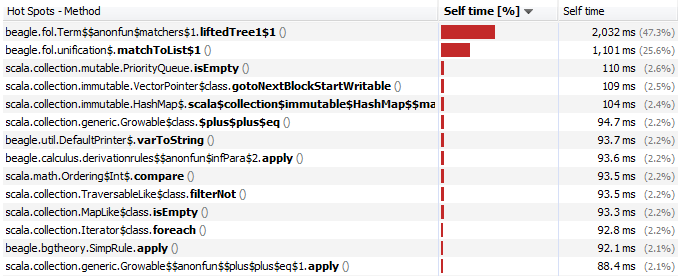
\includegraphics[width=\textwidth]{resources/visualvm}
  \caption{Typical results when instrumenting \beagle\  in VisualVM.}
  \label{fig:visvm}
\end{figure}

In the screenshot we can see there are two functions which together take up about
74\% of the total runtime. These two functions consistently took up most of \beagle's
computation time when VisualvM instrumentation was performed for a wide range of problems.
For readability the function names are re-stated here:
\begin{itemize}
\item[]beagle.fol.Term\$\$anonfun\$matchers\$1.\textbf{liftedTree\$1()}
\item[]beagle.fol.unification\$.\textbf{matchToList}\$1()
\end{itemize}
Knowing that these two functions take the most computation time does not immediately
help us with knowing the bottleneck which we must improve. To figure that out we must
trace the two functions back to where they are called from. We can see from the
names above that the first function is part of the Term Scala file (where Term objects and their
operations are defined) and the second is from the unification Scala file (a collection
of tools for performing unification and subsumption checks). Both functions are
used during the process of attempting to match or unify Term objects, a process
which is in turn only used during Superposition and Simplification. So we have confirmed
that \beagle's main bottleneck is part of these two operations; specifically when they attempt
to unify or match a great number of Terms. Thus by introducing Term Indexing
(which drastically reduces the number of Terms we attempt inference on) we will
be directly reducing strain on \beagle's most significant performance bottleneck.

\section{Problem Selection}
\label{sec:problems}

In order to test the performance of the completed implementation of Fingerprint Indexing
we will make use of problems from TPTP, the Thousands of Problems for Theorem Provers
library \cite{tptp}.
We will wish to compare many different versions of \beagle, making a full run of TPTP
for each version
exceedingly impractical; especially considering the available time and resources (\citeN{shulz12}
made use of the University of Miami \emph{Peagsus Cluster} to run his tests). Thus
we must select a subset of problems which we may perform our tests against.
This subset will consist of 50 TPTP problems across four problem categories.
\begin{itemize}
\item 10 \textbf{Arithmetic} (ARI) Problems. These problems are extremely relevant
to \beagle, as they allow it to make significant use of the integer arithmetic
background reasoning module. Unfortunately this makes ARI problems too easy for \beagle\ 
and most of them are solvable instantly without any foreground inferences. This makes
them completely irrelevant to indexing; hence we only include a selection of the 10 most complex ARI problems. 
\item 20 \textbf{Data} (DAT) Problems. Data problems are generally quite large and
require a large number of logical inferences to perform array manipulation operations.
This makes them perfect for testing Term Indexing.
\item 10 \textbf{Puzzle} (PUZ) Problems. Logic puzzles which are usually quite
complex but occasionally can be solved instantly.
\item 10 \textbf{Group Theory} (GRP) Problems. Usually quite complex but occasionally
boil down to modular arithmetic problems which are solved instantly by the background prover.
\end{itemize}
In selecting the problems above we must be \emph{fair} in the sense of not selecting
problems which favour indexing; but we also are not interested in problems where
indexing is not used. To achieve this we will select problems sequentially wherever
possible, which prevents us from picking out specific problems where indexing
performs exceptionally. Unfortunately in the case of the PUZ and GRP some problems had
to be skipped over due to being slight modifications of the previous problem, instantly solvable by all versions
or (in a few cases) not solvable by any version of \beagle. For a full
list of all the problems being tested against refer to Appendix \ref{app:app1}.

\section{Indexing Metrics}
\label{sec:metrics}

Before we may begin our test runs we must decide precisely what we are testing for, that is,
what we are using to measure \beagle's performance. In this section
we propose 3 major performance indicators, total run time, \emph{false positives} (for indexing)
and run time \emph{per inference}.

\subsection{Total Run Time}
\label{sec:runtime}

The most obvious performance metric for any program is run time or speed.
In order to measure time in our final test runs 
we will no longer be using VisualVM as in Section \ref{section:instr}. This program is well suited to our earlier task
of finding bottlenecks; but it will cause problems when attempting to analyse performance of a completed program.
In particular, attaching VisualVM to the Scala process will introduce significant overhead;
introducing variance and inaccuracy in our results. Furthermore, as we have seen in Section \ref{section:instr},
it can be difficult to determine how long is spent in each high-level inference rule
when we only see the computation time for bottom-level helper functions.

So, as an alternative to VisualVM we will instead perform all our timing manually
by injecting stopwatches into \beagle's code. This will allow us to directly
time each of the inference rules at the top level. For the purpose of our analysis
we will be timing 6 sections of \beagle:
\begin{itemize}
\item \textbf{Indexing}: Total time spent adding Terms to any of the Fingerprint Indices.
\item \textbf{Retrieving}: Total time spent retrieving Terms from any of the Fingerprint Indices.
\item \textbf{Superposition}: Total time spent performing Superposition (includes time spent
querying the index)
\item \textbf{Demodulation}: Total time spent performing Demodulation (includes time spent
querying the index)
\item \textbf{Negative Unit Simplification}: Total time spent performing Negative Unit Simplification (includes time spent
querying the index)
\item \textbf{Total}: Total time for the whole proof process. This \emph{does not} include
set-up time such as parsing and interpreting the input file and initial memory allocation.
\end{itemize}
At this point it is important to discuss the effectiveness of comparing totalled timing
results. While being the most intuitive measure of performance it can be misleading;
since (essentially through chance) different versions of \beagle\ will attempt logical
inferences in different orders. This can result in a version `getting lucky' and solving
a problem instantly where others get stuck. Thus in our results we will also include
a count for how many times each inference rule was used; which we may then take
into consideration when comparing results.

\subsection{False Positives}

A \emph{false positive} refers to a Term retrieved from a Fingerprint Index which does not
result in an applicable inference. Each false positive results in wasted computation;
making them a decent indicator of an Index's overall usefulness when solving a problem. That being said,
we must take a great deal of care in interpreting the false positive count, as
a low count does not necessarily indicate good overall performance. By na\"{\i}vley
boosting the size of the position sampling set it is possible to drop the false
positive count arbitrarily low; but this will result in an overcomplicated Index which
takes a long time to retrieve compatible Terms. Thus rather than strictly desiring a
low false positive count our goal for best performance is to balance the count with Fingerprint length.

In some initial testing, \beagle\ with indexing exhibited extremely high false positive
counts. After an email correspondence with Stephan \citeN{shulz12} these counts were determined
too high for Fingerprint Indexing to possibly be working correctly. After some analysis
it was determined that many thousands of Terms retrieved from the index successfully unified but failed to
perform a inference due to the large number of extra restrictions the \HSWAC places
on superposition (see Section \ref{sec:calc}). Thus the definition of a false positive
was slightly modified in \beagle\ to be a retrieved Term which does not successfully
\emph{unify}, no longer including any Terms which are cheaply discarded due to conditions
of the calculus. This allows \beagle's false positive count to be more comparable
to other indexing techniques based on the traditional superposition calculus.
Our test statistics will also include a count for the total number of terms retrieved
from Fingerprint Indices, from which subtracting the number of inferences will
give the original given definition of a false positive.

\subsection{Runtime Per Inference}

In Section \ref{sec:runtime} above we mentioned that total runtime can be misleading
due to ordering flukes; where a version of \beagle\ may perform better since it
arbitrarily performed a key inference early on. Thus a better performance indicator
is time spent \emph{per inference}, where we take the number of inferences required into
account. This metric gives us a direct and clear indication of performance which
(unlike the other metrics above) cannot be misinterpreted. Run time per inference
is the most relevant performance indicator and the core of what this project
has been trying to improve with Term Indexing.

Note that calculating the run time per inference does not require any additional code in \beagle. Since we
have total times and counts for each inference rule the runtime per inference can
be calculated after each test.

\section{Comparing Versions of \Beagle}
\label{sec:indexresults}

In this section we present results and analysis for performance against the TPTP
problems and metrics discussed in Section \ref{sec:metrics} above. We will perform
an in-depth comparison of three different versions of the prover:
\begin{itemize}
\item \textbf{Unmodified:} \beagle\ at the commencement of this project; without
any use of Fingerprint Indexing.
\item \textbf{Standard:} \beagle\ with the standard implementation of Fingerprint
Indexing; lacking our tailored optimisations from Section \ref{sec:tailored}. Both
Superposition and Simplification are indexed.
\item \textbf{Enhanced:} The full implementation described in this report; including
tailored optimisations.
\end{itemize}
Note that the performance of the two indexed versions can vary depending on what
positions we sample in order to generate Term Fingerprints. For the purpose of this
test we will have both the standard and the enhanced versions sample the following
positions:
  \[\epsilon,\  1,\  2,\  3,\  1.1,\  1.2\]
This set is named FP6M by \citeN{shulz12}, and it achieved the best performance in
his paper. The following Tables (\ref{tab:vercount} and \ref{tab:vertimes})
provide the totalled performance results for the three versions over the set of
50 selected problems (See Section \ref{sec:problems}). We will discuss these results
as a whole and then proceed to analyse results for specific problems; available in
Appendix \ref{app:app1}.

\begin{table}[H]\begin{center}
  \caption{Totalled inference counts and indexing statistics for various versions of \beagle.}
  \label{tab:vercount}
\begin{tabular}{| l || r | r | r || r | r | r |}  \cline{2-7}
\multicolumn{1}{ c }{} & \multicolumn{3}{ |c|| }{\textbf{Inference Counts}} & \multicolumn{3}{ c| }{\textbf{Indexing Results}} \\ \cline{1-7}
Version&Sup&Demod&NegUnit&TotalFound&SupFP&SimpFP\\  \cline{1-7}
\textbf{Unmodified \footnotemark[1]}&414216&29097&1826&0&0&0\\
\textbf{Standard}&162881&41414&2452&61884768&15525&39778148\\
\textbf{Enhanced}&146861&35326&1960&58119897&17641&39916687\\  \hline
\end{tabular}\end{center}\end{table}

\begin{table}[H]\begin{center}
  \caption{Totalled timing results for various versions of \beagle.}
  \label{tab:vertimes}
\begin{tabular}{| l || r | r | r | r | r | r |}  \cline{2-7}
\multicolumn{1}{ c }{} & \multicolumn{6}{| c| }{\textbf{Time Spent (seconds)}} \\ \cline{1-7}
Version&Indexing&Retrieving&Sup&Demod&NegUnit&Total\\  \cline{1-7}
\textbf{Unmodified \footnotemark[1]}&0&0&730.44&9.44&31.99&5623.21\\
\textbf{Standard}&28.4&38.73&254.17&41.66&3.18&381.36\\
\textbf{Enhanced}&18.74&17.58&168.79&30.56&2.12&259.02\\ \hline
\end{tabular}\end{center}\end{table}

\footnotetext[1]{This version failed to solve two problems within 8 hours (28800 seconds).
These results are not included in the totals. See verbose table of results (Section \ref{sec:unres})}

\subsection{Totalled Performance Against Indexing Metrics}
\label{sec:metricperf}

In this section we will discuss the results we see in the tables of total results
across the problem set (Tables \ref{tab:vercount} and \ref{tab:vertimes}); in
relation to the performance metrics we discussed in Section \ref{sec:metrics}.
Performance results for each individual problem are available in Appendix \ref{app:app1}
and will be discussed below in Sections \ref{sec:small} and \ref{sec:large}.

\subsubsection{Total Time}
Looking only at the final total runtime for the three programs it would appear as
though using indexing has resulted in an improvement of over 95\% from 5623 seconds
to 259. In addition to this, the unmodified version also failed to solve two
DAT problems entirely when given 8 hours (28800 seconds) to solve each one; and accounting
for these problems results in at least a 99.6\% improvement!
Unfortunately however this improvement cannot be entirely attributed to
our implementation of Fingerprint Indexing; and as mentioned in Section \ref{sec:metrics}
we must be careful to consider all factors. In particular, notice that the unmodified
version performs 414216 superposition inferences, nearly three times that of our
final enhanced implementation. This sort of discrepancy is not entirely unexpected,
and is essentially a fluke introduced by changing the order inferences are performed.
With this in mind the 95\% improvement is no longer relevant; and we must look into alternative
measures of performance.

Notice however that the standard version of beagle only performs about 10\% more
superposition inferences than the enhanced version; making these two versions much more comparable
on total time. Between these two versions we observe a total run time improvement
of 122 seconds, or about 2.5 seconds per problem. Of particular interest in comparing
these two versions is the difference between time spent retrieving from the index.
We notice that the enhanced version spends about 50\% less time performing retrievals;
even though it uses a far more complicated comparison table function (compare Listing
\ref{lst:unitable} for the standard version to Listing \ref{lst:extuni} for enhanced).
The speed up must then come from a reduced need to traverse the Fingerprint Index
due to less matching fingerprints; implying that our tailored improvements are greatly
improving the efficiency of Fingerprint Indexing.


\subsubsection{False Positives}
When we examine the count for false positives it does not immediately reflect our
above finding that the enhanced version has improved the efficiency of indexing.
In fact we observe over 10\% \emph{more} superposition false positives in the enhanced
version (and about 0.5\% more simplification false positives). This seems to contradict
our raw timing results; but the contradiction may be resolved by considering all factors involved.

An indexing false positive obviously results in some unnecessary computation as we
have attempted unification and failed. However, even after unification succeeds we may
still fail to perform superposition due to other restrictions of the inference rule.
In particular there are four Literal and Term ordering restrictions which must
be checked \emph{after} verifying unification, as they require the substitution
used (see Section \ref{sec:calc}). This means that even when a term
is not counted as a false positive for unification it may still cause the same
amount of unnecessary computation.

Thus we must consider the TotalFound column, which counts the total number of terms
retrieved from the index; regardless of whether or not they result in unification or an inference.
In this column we observe a superb improvement in the enhanced version
of \beagle, with it retrieving almost four million fewer terms than the standard index.
This difference is direct evidence of tailored enhancements reducing the amount of index traversal necessary;
and unlike the false positive count we can be sure that each term not retrieved
is saving us some amount of computation. This explains how we can have 2116 more
false positives and still see a significant increase in performance; but we still
have not seen how these extra false positives could have occurred.

The difference is small enough that we can again consider it a fluke arising from
the variation in inference order. This is very unsatisfying however since our
improved unification table from Section \ref{sec:extunif} should result specifically
in fewer false positives; not just fewer terms retrieved from the index. 
Recall that the extended table works by considering the placement of terms
in the hierarchy (whether they are foreground or background). Thus the improvement will only
be relevant when there are a reasonable percentage of background terms; such as in
arithmetic problems.
When examining only the set of ten ARI problems 
(see the verbatim result tables in Appendix \ref{app:app1}) we observe
that the enhanced version is superior by all measures of performance.
In fact we observe a total of \emph{zero}
superposition false positives versus 124 for the standard version. This result shows the true worth of our
improved unification table, as it is not necessarily relevant in the case of DAT, PUZ
and GRP problems. Our additional tailored improvements from Section \ref{sec:otherimp}
are still relevant for these problems and produce the significant improvement
seen in total terms retrieved.

\subsubsection{Time Per Inference}

Now we come to what is perhaps the most relevant and telling measure of performance;
\emph{time spent per inference}. This measure is not affected by any random factors
introduced by changing the order of inference and gives us a true indication of how
much we have improved each inference rule. Table \ref{tab:peri} presents the results
for this performance measure; derived from the totals above.

 \begin{table}[H]\begin{center}
  \caption{Total time spent per inference for various versions of \beagle.}
  \label{tab:peri}
\begin{tabular}{| l || r | r | r |}  \hline
Version&Superposition&Demodulation&NegUnit Simplification\\  \hline
\textbf{Unmodified}&1.7ms & 0.3ms & 17.5ms  \\
\textbf{Standard}  &1.5ms & 1.0ms & 1.3ms  \\
\textbf{Enhanced}  &1.1ms & 0.8ms & 1.0ms  \\\hline
\end{tabular}\end{center}\end{table}  

First of all we notice that the standard version of Fingerprint Indexing has
improved superposition by 2 milliseconds per inference, a 12\% improvement,
and our enhanced version has improved it by 6 milliseconds, a 35\% improvement.
While this is a far call from the 95\% improvement which total run time initially
implied it still presents a fantastic final result. Negative Unit Simplification
produces a phenomenal 94\% improvement, down to 1 millisecond per simplification from 17.5
(we will examine how this improvement occurred when examining individual problem
results in Section \ref{sec:large}).
Unfortunately demodulation does not produce the positive results we see in the other
inference rules and in fact our indexed versions perform far worse than the original
version of \beagle.

To explain this unfortunate result we refer again to the verbatim results in
Appendix \ref{app:app1}. In particular observe the results for problem PUZ037-1.p.
In the results for both the standard indexing and enhanced indexing versions of \beagle\ 
this problem takes up about 60\% of the total time spent on demodulation. Despite
this, not a single demodulation inference is performed; resulting in over \emph{38 million}
false positives for indexing simplification (which constitutes over 95\% of the
total simplification false positives for both versions). This puzzle seems to present
a `worst case scenario' for demodulation indexing and produces results far outside the norm.
Thus it is reasonable to exclude it as an outlier and consider demodulation results
without this problem included.

When excluding PUZ037-1.p we observe 0.29, 0.39 and 0.31 milliseconds per demodulation
for the unmodified, standard and enhanced versions respectively. Even though we no
longer see the significant loss of performance from Table \ref{tab:peri}, our
indexed versions are still performing slightly worse than original \beagle. Realistically
they are performing about the same; considering a 0.1 millisecond margin of error. Unfortunately
it seems as though \beagle's current implementation of demodulation is not well suited
to indexing. This is perhaps due to the fact that demodulation must still loop
over all subterms of its query Clause; but avoiding this would require very significant
modification to \beagle's main loop (as simplification currently only applies to
the Clause selected from \verb!new!, see Section \ref{sec:mloop} and \ref{sec:demod}).
On the other hand it is possible that the issue arises simply from
the specific problem set we are testing against; since in many of results we observe
very few or even zero demodulation operations. More testing is required to determine
if restructuring \beagle\ to improve demodulation could be worthwhile.


\subsection{Results for Small Problems}
\label{sec:small}

Here we shall present some results for the smaller problems in our TPTP selection.
A significant portion of the problems in TPTP are fairly small scale; and this
is reflected in our results where 42 out of the 50 problems take less than
10 seconds to solve in our final indexed version. It is interesting to take a
closer look at these small scale problems because they are where we should expect to see
indexing perform \emph{the worst}. In small, fast problems where our knowledge base is small
and few inferences are necessary we would expect indexing to be unnecessary and
only introduce complexity. Figure \ref{fig:worst} presents the superposition runtime
of all versions for problems where this time was less than 5 seconds; which makes up 43
of our 50 problems. The results
are presented in order of superposition time for unindexed \beagle.

\begin{figure}[h]
  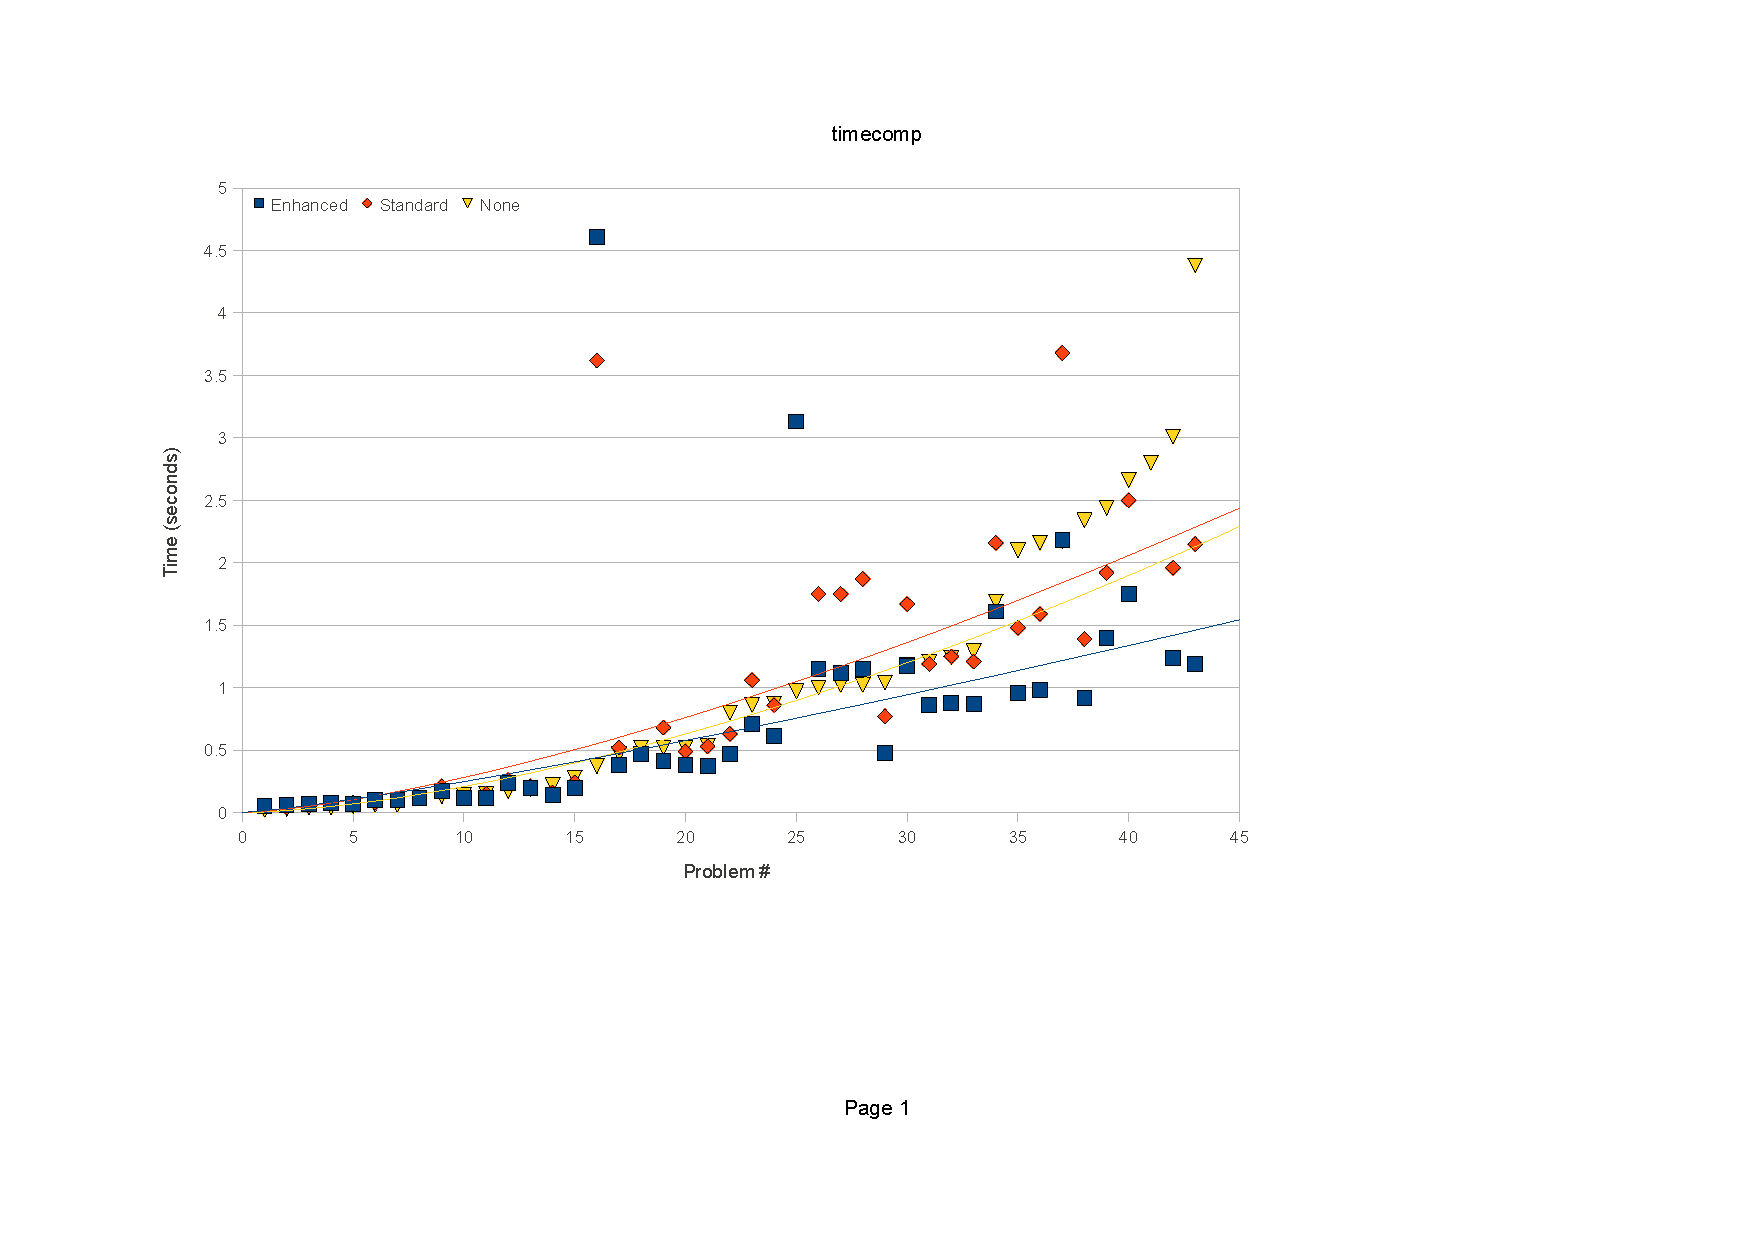
\includegraphics[trim=2.45cm 6cm 8cm 3cm,clip,width=\textwidth]{resources/suptimetrends}
  \caption{Superposition time comparison for three versions of \beagle\ for small problems
  (under 5 seconds of superposition).}
  \label{fig:worst}
\end{figure}

As expected, indexing does not achieve the 35-95\% improvement which
we have observed for the whole problem set. Up until about problem 33, where
the unindexed time goes over 1.5 seconds, the indexed versions of \beagle\ typically
perform about the same or worse than the unindexed version. After this point we
begin to see indexing provide a notable improvement; particularly in our enhanced
version. By inserting trend lines we can see that original \beagle\ and the standard
indexing version of beagle are achieving similar performance overall; and our enhanced
version begins to come out on top after about problem 30. This shows us that
even though indexing would not normally apply to these simple problems our tailored
optimisations have made it worthwhile.

\subsection{Results for Large Problems}
\label{sec:large}

More relevant to indexing performance are the results of large problems. When our
knowledge base consists of several thousand Clauses it no longer becomes practical
to search through them for inference matches and Term indexing becomes far more vital.
Furthermore for each inference we perform our knowledge base grows and this problem will become worse.
In this section we will discuss the results of large problems where many thousands of
inferences are performed; in which we expect Fingerprint Indexing to improve performance
significantly.

\subsubsection{Most Significant Superposition Results}

First of all we will examine the problems for which a significant amount of time
is spent on superposition. These problems make up the 7 out of 50 problems which
we did not consider in Section \ref{sec:small}. Table \ref{tab:bigsup} shows the
superposition count and timing results for these 7 problems against all 3 versions
of \beagle; sorted in order of time spent in the unindexed version.

 \begin{table}[H]\begin{center}
  \caption{Superposition counts and time for the 7 most extreme problem examples.}
  \label{tab:bigsup}
\begin{tabular}{| l || r | r || r | r || r | r |} \cline{2-7}
\multicolumn{1}{ c }{} & \multicolumn{2}{ |c|| }{\textbf{Enhanced}} & \multicolumn{2}{ c|| }{\textbf{Standard}} & \multicolumn{2}{ c| }{\textbf{Unmodified}} \\ \cline{1-7}
Problem&Sup Count&Sup Time&Sup Count&Sup Time&Sup Count&Sup Time\\  \hline
PUZ038-1.p& 2656   &24.59&  2656   &33.30 & 2579   & 22.6\\
DAT050=1.p& 52438  &17.53&  65908  &31.54 & 111277 & 48.62\\
DAT039=1.p& 11249  &13.20&  11278  &22.51 & 63897  & 130.77\\
DAT040=1.p& 10551  &14.49&  11765  &21.29 & 73775  & 190.71\\
DAT038=1.p& 10344  &12.53&  11848  &24.04 & 132216 & 294.86\\
DAT043=1.p& 15422  &18.67&  12865  &26.08 & \textbf{N/A}\footnotemark[1] & \textbf{N/A}\footnotemark[1] \\
DAT048=1.p& 14186  &17.65&  16462  &35.77 & \textbf{N/A}\footnotemark[1] & \textbf{N/A}\footnotemark[1] \\ \hline
\end{tabular}\end{center}\end{table}

\footnotetext[1]{These results are not included as the problem could not be solved within 8 hours (28800 seconds).}

Of particular note are the two final problems, which the original version of \beagle\ 
was unable to solve and timed out after 8 hours. In our final enhanced version these two problems
also present some of the largest times for superposition inferences; but in this case
they are no longer than \emph{twenty seconds}. This can
be partially considered a fluke of inference ordering; but without the ability
to rapidly apply inferences with indexing it would not have been possible to reach
the key inferences which allowed the problem to be solved.

\subsubsection{Most Significant Negative Unit Simplification Results}

Back in Section \ref{sec:metricperf} we observed a 94\% improvement for each
Negative Unit Simplification performed, down to 1 millisecond per simplification from 17.5. We will
now look at the problems which most stress the Negative Unit Simplification rule
and attempt to explain this tremendous performance increase. Looking at verbatim
results from Appendix \ref{app:app1} we can observe that there are four problems
from DAT for which Negative Unit Simplification takes an abnormally large portion
of time. In fact, for unindexed \beagle\ these four problems
cover over 97\% of the time spent performing Negative Unit Simplification! Table
\ref{tab:bigneg} lists the four problems along with their performance in the
three versions of the prover.

 \begin{table}[H]\begin{center}
  \caption{Negative Unit Simplification counts and time for the 4 most extreme problem examples.}
  \label{tab:bigneg}
\begin{tabular}{| l || r | r || r | r || r | r |} \cline{2-7}
\multicolumn{1}{ c }{} & \multicolumn{2}{ |c|| }{\textbf{Enhanced}} & \multicolumn{2}{ c|| }{\textbf{Standard}} & \multicolumn{2}{ c| }{\textbf{Unmodified}} \\ \cline{1-7}
Problem&Neg Count&Neg Time&Neg Count&Neg Time&Neg Count&Neg Time\\  \hline
DAT039=1.p&15&0.14&15&0.2&73&4.84\\
DAT040=1.p&17&0.13&16&0.2&81&5.94\\
DAT050=1.p&1743&0.71&2252&1.33&1414&6.24\\
DAT038=1.p&10&0.14&10&0.19&104&14.05\\\hline
\end{tabular}\end{center}\end{table}

The most interesting example problem here is DAT038=1.p, where we can see the unmodified
version spends an enormous amount of time checking for Negative Unit Simplifications;
but in the end performs comparatively few. This problem must have generated a large
number of negative unit Clauses which were not necessarily applicable for
Negative Unit Simplification; resulting in a great deal of unnecessary computation
for unindexed \beagle. In terms of time spent per inference, 
unindexed \beagle requires 135 milliseconds for each simplification;
which is nearly \emph{eight times} its norm. It is worth noting at this point that DAT038=1.p \emph{is not} a lone outlier; and
in particular we see very similar (though not quite as extreme) results in DAT039=1.p and DAT040=1.p.
These problems are also made relevant by the fact that our indexed versions are suffering
from the same issue of excessive negative unit Clause generation.
However, they are much more capable of coping with large quantities of negative Literals.
As a result they do see worse than average simplification times here but perform
far better than unindexed \beagle. 

\section{Comparing Various Fingerprint Sampling Positions}
\label{sec:fingcomp}

Now that we have thoroughly explored and compared the three different versions of
\beagle\ it is now worth considering the impact of different Fingerprint Indexing
configurations; in particular the set of positions being sampled. 
By increasing the number of positions sampled we should
expect a decrease in false positive rate, since Terms retrieved from the Index will
be compatible for unification at more points. Unfortunately however this does
not necessarily correspond to an increase in overall performance.
The set of positions determines how long each Term Fingerprint is and thus decides the depth of our Index
tree (See Section \ref{sec:fpindex}). With a more complex Index structure each
retrieval of compatible Terms will take more computation and more time. It is
therefore important that we strike a balance between accurate comparisons and
quick comparisons.

\pagebreak

A wide variety
of sampling configurations was tested by \citeN{shulz12}, so our primary goals
here are to cross-reference our results with his and confirm which set best balances Fingerprint length.
For this purpose we will compare 6 of the best performing sampling sets proposed by
Shulz. The sets we will be comparing are as follows: (see Section \ref{sec:terminology}
for an explanation of position syntax)

  \begin{itemize}
  \item FP3W: Samples 3 positions to a maximum depth of 2. While this set creates
  tiny Fingerprints it was still able to achieve good results due to the relative simplicity
  of retrieving from the index. \cite{shulz12}
  \[\epsilon,\  1,\  2\]
  \item FP4M: Samples 4 positions to a maximum depth of 3.
  \[\epsilon,\  1,\  2,\  1.1\]
  \item FP6M: Samples 6 positions to a maximum depth of 3. This set produced the
  best performance in the tests by \citeN{shulz12}, and was used for the version
  comparisons in Section \ref{sec:indexresults}.
  \[\epsilon,\  1,\  2,\  3,\  1.1,\  1.2\]
  \item FP7: Samples 7 positions to a maximum depth of 3.
  \[\epsilon,\  1,\  2,\  1.1,\  1.2,\  2.1,\  2.2\]
  \item FP8X2: Samples 16 positions. This is an example of excessively large Fingerprints
  which should result in a steep decrease in performance.
  \[\epsilon,\  1,\  2,\  3,\  4,\  1.1,\  1.2,\  1.3,\  2.1,\  2.2,\  2.3,\  3.1,\  3.2,\  3.3,\  1.1.1,\  2.1.1\]
  \end{itemize}


Tables \ref{tab:fingcount} and \ref{tab:fingtime} provide the total performance
for each Fingerprint sampling set. These totals are taken over \emph{49} of our
50 problems. PUZ037-1.p has been excluded from these results since (as we discussed
in Section \ref{sec:metricperf}) it presents an exceptional `worst case' for demodulation
indexing; making results including it difficult to compare (particularly for simplification
false positives). Verbatim results for each problem along with total results over all
50 problems are available in Appendix \ref{app:app2}.

\pagebreak

\begin{table}[H]\begin{center}
  \caption[]{Totalled inference counts and indexing statistics for various Fingerprint sampling sets.\footnotemark[1]}
  \label{tab:fingcount}
\begin{tabular}{| l || r | r | r || r | r | r |}  \cline{2-7}
\multicolumn{1}{ c }{} & \multicolumn{3}{ |c|| }{\textbf{Inference Counts}} & \multicolumn{3}{ c| }{\textbf{Indexing Results}} \\ \cline{1-7}
Sample Set&Sup&Demod&NegUnit&TotalFound&SupFP&SimpFP\\  \cline{1-7}
\textbf{FP3W}&162218&42402&2472&13913606&69429&1815992\\
\textbf{FP4M}&147798&35709&1963&13469779&26847&1851515\\
\textbf{FP6M}&144505&35326&1959&12601762&16406&1694731\\
\textbf{FP7}&160641&41435&2453&13017546&14166&1557268\\
\textbf{FP8X2}&159385&40876&2438&12819184&11229&1602033\\ \hline 
\end{tabular}\end{center}\end{table}

\begin{table}[H]\begin{center}
  \caption[]{Totalled timing results for various Fingerprint sampling sets.\footnotemark[1]}
  \label{tab:fingtime}
\begin{tabular}{| l || r | r | r | r | r | r |}  \cline{2-7}
\multicolumn{1}{ c }{} & \multicolumn{6}{| c| }{\textbf{Time Spent (seconds)}} \\ \cline{1-7}
Sample Set&Indexing&Retrieving&Sup&Demod&NegUnit&Total\\  \cline{1-7}
\textbf{FP3W}&11.52&14.02&170.37&9.26&1.78&237.75\\
\textbf{FP4M}&13.09&14.12&164.95&9.51&1.82&230.68\\
\textbf{FP6M}&16.82&16.5&159.93&10.78&2.11&229.59\\
\textbf{FP7}&20.62&19.22&170.89&12.55&2.5&250.8\\
\textbf{FP8X2}&45.56&32.59&181.43&21.45&4.06&294.8\\ \hline 
\end{tabular}\end{center}\end{table}

\footnotetext[1]{Excludes problem PUZ037-1.p}

False positives are the main statistic we expect to be impacted by altering
position sets. Notice that when only sampling 3 positions we see a huge number
of superposition false positives, which more than halves when we move up to the FP4M set. Each
extra position we sample drops the superposition false positive count further;
though no other drops are as significant as the drop when moving from 3 positions to 4.
The false positives for simplification are also on a falling trend; but not quite as
consistently or uniformly as the false positives for superposition.

Recall that a decrease in false positives does not necessarily imply a decrease
in performance. Consider the difference between time results for FP3W and FP4M. Sampling
an extra position only saves us about 5 seconds of superposition time; despite the
fact that we cut false positives in half. This trend continues when we add two positions
to FP6M. Between FP4M and FP6M we observe a saving of 5 seconds during superposition;
but after the extra time required to index and retrieve terms we only save just over
a second in total runtime. After 6 positions the trend of gentle performance increase
reverses; and as expected we have reached a point where increasing indexing accuracy
is no longer worthwhile. On the extreme far end of the scale where we sample 16
positions (FP8X2) overall performance has dropped significantly. Even though FP8X2
has a sixth the amount of false positives that FP3W has it takes nearly a minute
longer to solve all 49 problems.

These results line up with our expectations for how Fingerprint lengths impact
performance; and with the results from \cite{shulz12}. Like Shulz, our best result
was given by FP6M. It is only the best set by a very small margin however; and
both tests of smaller sets perform essentially the same if we consider a reasonable
margin of error. It would appear as though the set used for Fingerprint Indexing
does not have a significant impact on performance so long as Fingerprint length
is kept within a range of about 3 to 6.

There is another interesting phenomenon in these results which we have not yet discussed.
The total time spent on both simplification rules
(Demodulation and Negative Unit Simplification) gets uniformly worse as we add
sampling positions; quite significantly in the case of Demodulation. Notice that
regardless of how many positions we sample we always observe a large count for 
simplification false positives; with only a 12\% decrease from FP3W to FP8X2.
This implies that the extra sampling positions are not as useful for simplification
indexing, resulting in us only observing the loss of performance from complicating
Term retrieval. This is possibly due to the fact that for simplification we
only ever index unit Clauses; which will often be quite simple compared to the
wide array of Terms seen in the superposition index. Smaller terms are less likely
to be able to make use of more sampling positions, which would explain why adding
them does not result in increased performance.

%%% Local Variables: 
%%% mode: latex
%%% TeX-master: "thesis"
%%% End: 
